%{{{ Formatierung

\documentclass[a4paper,10pt]{article}

\usepackage{physics_notetaking}

%%% dark red
%\definecolor{bg}{RGB}{60,47,47}
%\definecolor{fg}{RGB}{255,244,230}
%%% space grey
%\definecolor{bg}{RGB}{46,52,64}
%\definecolor{fg}{RGB}{216,222,233}
%%% purple
%\definecolor{bg}{RGB}{69,0,128}
%\definecolor{fg}{RGB}{237,237,222}
%\pagecolor{bg}
%\color{fg}

\newcommand{\td}{\,\text{d}}
\newcommand{\RN}[1]{\uppercase\expandafter{\romannumeral#1}}
\newcommand{\zz}{\mathrm{Z\kern-.3em\raise-0.5ex\hbox{Z} }}
\newcommand{\id}{1\kern-.258em1}

\newcommand\inlineeqno{\stepcounter{equation}\ {(\theequation)}}
\newcommand\inlineeqnoa{(\theequation.\text{a})}
\newcommand\inlineeqnob{(\theequation.\text{b})}
\newcommand\inlineeqnoc{(\theequation.\text{c})}

\newcommand\inlineeqnowo{\stepcounter{equation}\ {(\theequation)}}
\newcommand\inlineeqnowoa{\theequation.\text{a}}
\newcommand\inlineeqnowob{\theequation.\text{b}}
\newcommand\inlineeqnowoc{\theequation.\text{c}}

\renewcommand{\refname}{Source}
\renewcommand{\sfdefault}{phv}
%\renewcommand*\contentsname{Contents}

\newenvironment{Figure}
        {\par\medskip\noindent\minipage{\linewidth}}
        {\endminipage\par\medskip}

\pagestyle{fancy}

\sloppy

\numberwithin{equation}{section}

%}}}

\begin{document}

%{{{ Titelseite

\begin{titlepage}
        \title{5 (1.\ Halbtag) $|$ Operationsverstärker}
        \author[1]{Angelo Brade\thanks{s72abrad@uni-bonn.de}}
        \author[1]{Jonas Wortmann\thanks{s02jwort@uni-bonn.de}}
        \affil[1]{Rheinische Friedrich--Wilhelms--Universität Bonn}
        \date{\today}
\end{titlepage}

\maketitle
\pagenumbering{gobble}

%}}}

\newpage

%{{{ Inhaltsverzeichnis

\fancyhead[R]{\leftmark}
%\fancyhead[R]{\leftmark\\\rightmark}
\fancyhead[L]{\thepage}
\fancyfoot[C]{}

\tableofcontents

%}}}

\clearpage

%{{{

\pagenumbering{arabic}

\begin{multicols}{2}

        \section{Introduction}

        \section{Theory}

        \section{Preliminary Tasks}
        \subsection{A}
        The equation hold
        \begin{align} 
                \dfrac{1}{\nu }&=\dfrac{1}{\nu _0}+k&\nu &=\dfrac{1}{\tfrac{1}{\nu _0}+k}
        .\end{align} 
        For $k=0.1$, $\nu _0=10^4$ and $\nu _0=10^5$
        \begin{align} 
                \nu _1&\approx 9.990 & \nu _2&\approx 9.999
        .\end{align} 
        The approximation $\nu =\tfrac{1}{k}$ results in
        \begin{align} 
                \nu _\text{Näh}&=10
        .\end{align} 
        The deviation of $\nu _1$ and $\nu _2$ from $\nu _\text{Näh}$ lie at $0.001\%$ and $0.0001\%$ respectively.

        \subsection{B}
        It hold
        \begin{align} 
                &&&& U_x &= U_\text{in}-kU_\text{out} &&&& \\
                &&\Leftrightarrow && &= U_\text{in}-kv_0U_x &&&&\nonumber \\
                &&\Leftrightarrow && &= \dfrac{U_\text{in}}{1+v_0k}. &&&&
        \end{align} 
        For $k=0.1$, $v_0=10^5$ and $U_\text{in}=\SI{1}{V}$
        \begin{align} 
                U_x\approx \SI{0.0001}{V}
        .\end{align} 

        \subsection{C}
        Let there be a common mode signal with $\Delta U_+=\Delta U_-=+\Delta U_\text{in}$.
        then
        \begin{align} 
                &&&& \Delta U_+ &= \Delta U_E+\Delta U_1 & \Delta U_- &= \Delta U_E+\Delta U_1. &&&& 
        \end{align} 
        from this follows $\Delta U_\text{in}=\Delta U_E+\Delta U_1$.
        The output voltage is
        \begin{align} 
                \Delta U_\text{out}=R_C\cdot \Delta I_C
        .\end{align} 
        At point 1,
        \begin{align}
                I_1=2I_E
        .\end{align} 
        Therefore
        \begin{multline} 
                \Delta U_\text{in} = R_E\cdot \Delta I_E+R_1 \cdot 2\Delta I_E \\= \Delta I_E\left(R_E+2R_1\right)\approx \Delta I_E\cdot 2R_1.
        \end{multline} 
        At the node $U_\text{out}$ applies
        \begin{align} 
                \Delta I_E=\Delta I_C\Rightarrow \Delta U_\text{out}=R_C\cdot \Delta I_E
        .\end{align} 
        The amplification results in
        \begin{align} 
                v_{CM}=\dfrac{\Delta U_\text{out}}{\Delta U_\text{in}}=\dfrac{R_C}{2R_1}
        .\end{align} 
        The common mode suppression is
        \begin{align} 
                10\log \left(\dfrac{R_E}{R_1}\right)=10\log \left(\dfrac{\SI{1}{\kilo\ohm}}{\SI{100}{\kilo\ohm}}\right)=-\SI{20}{dB}
        .\end{align} 

        \subsection{D}
        The frequency dependence of the impedance of a capacitor is
        \begin{align} 
                Z_1 &= \dfrac{1}{\text{i}\omega C}=\dfrac{1}{\text{i}2\pi fC}\\
                |Z_1| &= \left|\dfrac{1}{\text{i}\omega C}\right| = \dfrac{1}{2\pi fC}
        .\end{align} 
        The gain as a function of frequency is
        \begin{align} 
                v\left(f\right)=1+\dfrac{Z_2}{|Z_1|}=1+R2\pi fC
        .\end{align} 
        The limits are
        \begin{align} 
                \lim_{f \rightarrow 0}\left[1+R2\pi fC\right] &= 1 & \lim_{f \rightarrow \infty}\left[1+R2\pi fC\right] &= \infty
        .\end{align} 
        For $|Z_1| = R$ it has to hold that
        \begin{align} 
                \dfrac{1}{2\pi fC}=R\Leftrightarrow f=\dfrac{1}{2\pi RC}
        .\end{align} 
        With concrete values $Z_1=R=\SI{100}{\kilo\ohm}$ and $Z_1=C=\SI{100}{\nano F}$, the frequency is
        \begin{align} 
                f=\dfrac{1}{2\pi RC}\approx \SI{15.92}{Hz}\Rightarrow v\left(f\right)\approx 2
        .\end{align} 
        \begin{Figure}
                \centering
                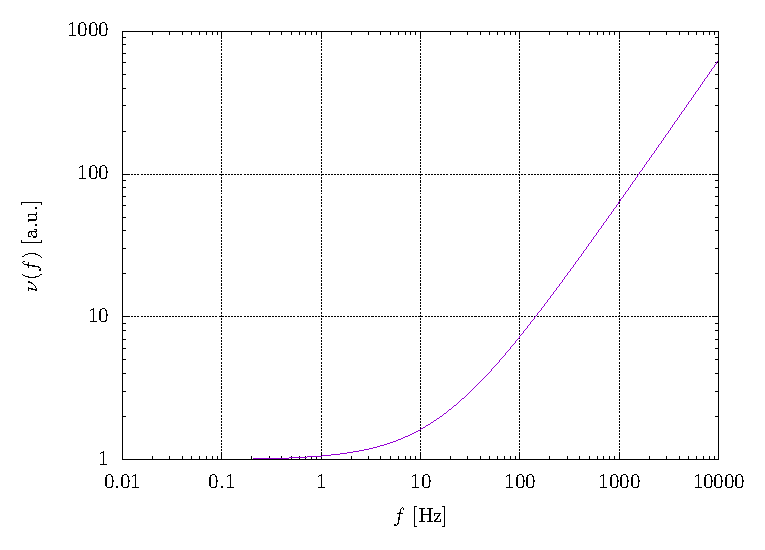
\includegraphics[width=0.7\textwidth]{../plot/preE_crop.pdf}
                \captionof{figure}{Time dependend amplification of a non--invertible amplifier as a \textsc{Bode}--plot}
        \end{Figure}

        \subsection{E}
        Let
        \begin{align} 
                v=\dfrac{U_\text{out}}{U_\text{in}}=-\dfrac{Z_2}{Z_1}
        .\end{align} 
        The minus sign results from the negative feedback.
        Because of the golden rule $U_-=U_+=\SI{0}{V}$, the negative feedback has a different sign compared to the input signal.
        \\\indent The input impedance is very high and the output impedance very low. 

        \subsection{F}
        

        \newpage
        \section{Auswertung}
\end{multicols}

\clearpage
\listoffigures
\listoftables
\bibliographystyle{plain}
\bibliography{refs}

%}}}

\end{document}
